\documentclass{standalone}

\usepackage{tikz}
\usetikzlibrary{calc}

\begin{document}

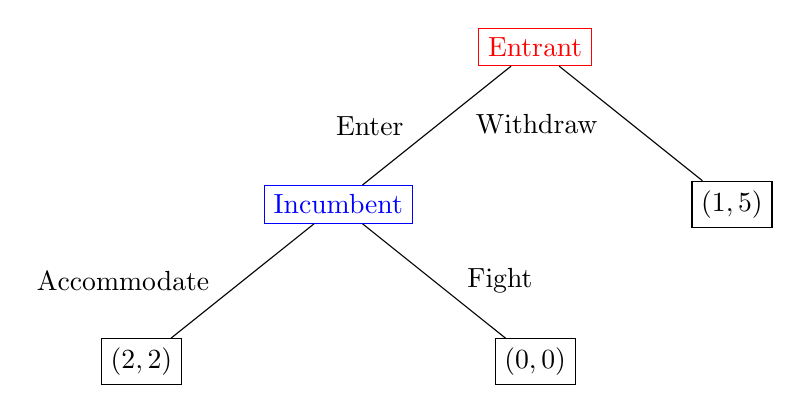
\begin{tikzpicture}
    \node [draw, color=red] (A) at (0, 0) {Entrant};
        \node [draw, color=blue] (B) at ($(A) + (-2.5, -2)$) {Incumbent};
        \node [draw] (O1) at ($(A) + (2.5, -2)$) {$(1, 5)$};
        \node [draw] (O3) at ($(B) + (-2.5, -2)$) {$(2, 2)$};
        \node [draw] (O2) at ($(B) + (2.5, -2)$) {$(0, 0)$};
    \draw (A) -- node[left=3mm] {Enter} (B);
    \draw (A) -- node[left=3mm] {Withdraw} (O1);
    \draw (B) -- node[left=3mm] {Accommodate} (O3);
    \draw (B) -- node[right=3mm] {Fight} (O2);
\end{tikzpicture}

\end{document}
